%%
%% This is file `example.tex',
%% generated with the docstrip utility.
%%
%% The original source files were:
%%
%% coppe.dtx  (with options: `example')
%% 
%% This is a sample monograph which illustrates the use of `coppe' document
%% class and `coppe-unsrt' BibTeX style.
%% 
%% \CheckSum{1416}
%% \CharacterTable
%%  {Upper-case    \A\B\C\D\E\F\G\H\I\J\K\L\M\N\O\P\Q\R\S\T\U\V\W\X\Y\Z
%%   Lower-case    \a\b\c\d\e\f\g\h\i\j\k\l\m\n\o\p\q\r\s\t\u\v\w\x\y\z
%%   Digits        \0\1\2\3\4\5\6\7\8\9
%%   Exclamation   \!     Double quote  \"     Hash (number) \#
%%   Dollar        \$     Percent       \%     Ampersand     \&
%%   Acute accent  \'     Left paren    \(     Right paren   \)
%%   Asterisk      \*     Plus          \+     Comma         \,
%%   Minus         \-     Point         \.     Solidus       \/
%%   Colon         \:     Semicolon     \;     Less than     \<
%%   Equals        \=     Greater than  \>     Question mark \?
%%   Commercial at \@     Left bracket  \[     Backslash     \\
%%   Right bracket \]     Circumflex    \^     Underscore    \_
%%   Grave accent  \`     Left brace    \{     Vertical bar  \|
%%   Right brace   \}     Tilde         \~}
%%
\documentclass[grad,numbers]{coppe}
\usepackage{amsmath,amssymb}
\usepackage{hyperref}
\usepackage[utf8]{inputenc}
\usepackage[brazil]{babel}
\usepackage[T1]{fontenc}
\usepackage{graphicx}
\usepackage{amsmath}
\usepackage{minted}

\makelosymbols
\makeloabbreviations

\begin{document}
  \title{Técnicas de Aprendizado de Máquina aplicadas a AlgoTrading no Mercado de Ações}
  \foreigntitle{Machine Learning Techniques applied to AlgoTrading in the Stock Market}
  \author{Lucas}{Schlee de Brito Fernandes}
  \advisor{Prof.}{Heraldo}{Luís Silveira de Almeida}{D.Sc.}
  \advisor{Prof.}{Flávio}{Luis de Mello}{Ph.D.}

  \examiner{Prof.}{Nome do Primeiro Examinador Sobrenome}{D.Sc.}
  \examiner{Prof.}{Nome do Segundo Examinador Sobrenome}{Ph.D.}
  \examiner{Prof.}{Nome do Terceiro Examinador Sobrenome}{D.Sc.}
  \examiner{Prof.}{Nome do Quarto Examinador Sobrenome}{Ph.D.}
  \examiner{Prof.}{Nome do Quinto Examinador Sobrenome}{Ph.D.}
  
  
  
  \department{ECA}% Confira a tabela a seguir para saber como preencher o comando \department de acordo com seu curso (Graduação - Poli) ou programa (Pós-Graduação - COPPE).
  
  %%%%%% Para alunos da POLI %%%%%%
  
  %% Course											Option
  %% Engenharia Ambiental                             EA
  %% Engenharia Civil                                 ECV
  %% Engenharia de Computação e Informação            ECI
  %% Engenharia de Controle e Automação               ECA
  %% Engenharia de Materiais                          EMAT
  %% Engenharia de Petróleo                           EPT
  %% Engenharia de Produção                           EPR
  %% Engenharia Eletrônica e de Computação            EEC
  %% Engenharia Elétrica                              EET
  %% Engenharia Mecânica                              EMC
  %% Engenharia Metalúrgica                           EMET
  %% Engenharia Naval e Oceânica                      ENO
  %% Engenharia Nuclear                               ENU
  
  
  %%%%%% Para alunos da COPPE %%%%%%
  
  %% Program											Option
  %% Engenharia Biomédica								PEB
  %% Engenharia Civil									PEC
  %% Engenharia Elétrica								PEE
  %% Engenharia Mecânica								PEM
  %% Engenharia Metalúrgica e de Materiais				PEMM
  %% Engenharia Nuclear									PEN
  %% Engenharia Oceânica								PENO
  %% Planejamento Energético							PPE
  %% Engenharia de Produção								PEP
  %% Engenharia Química									PEQ
  %% Engenharia de Sistemas e Computação				PESC
  %% Engenharia de Transportes							PET
  
  
  
  
  
  
  \date{02}{2019}

  \keyword{Aprendizado de Máquina}
  \keyword{Mercado Financeiro}
  \keyword{Algotrading}

  \maketitle

  \frontmatter
  
  \makecatalog
  
  \dedication{A alguém cujo valor é digno desta dedicatória.}

  \chapter*{Agradecimentos}

  Gostaria de agradecer a todos.

  \begin{abstract}

  A cada dia no mercado de ações é possível identificar milhares de decisões tomadas automaticamente, sem a necessidade de intervenção humana. Apesar disso, essa tendência, considerada irreversível, ainda utiliza estratégias baseadas em regras bem definidas. Nesse contexto, o presente trabalho propõe a aplicação de técnicas de aprendizado de máquina para identificar padrões e prever a direção dos preços das ações para negociações de alta frequência.

  \end{abstract}

  \begin{foreignabstract}

  Each day in the stock market it`s possible to identify thousands of decisions made automatically, without the need for human intervention. Despite this, this trend, considered irreversible, still uses strategies based on well-defined rules. In this context, the present work proposes the application of machine learning techniques to identify patterns and predict the direction of stock prices for high frequency trades.

  \end{foreignabstract}

  \tableofcontents
  \listoffigures
  \listoftables
  \printlosymbols
  \printloabbreviations

  \mainmatter
%  \doublespacing
\chapter{Introdução}
  
  \section{Tema}
    
    \paragraph{}O projeto consiste na aplicação de inteligência articificial às negociações de alta frequência no mercado financeiro (\textit{High Frequency Trading}). Nesse contexto, o problema a ser resolvido é o levantamento de padrões de mercado que indiquem uma previsão futura, a curto prazo, de uma variação positiva no preço de um determinado ativo.
    
  \section{Delimitação}

    \paragraph{}Toda a base de dados construída para o presente trabalho foi proveniente dos dados reais negociados na Bolsa de Valores de São Paulo (BM\&FBOVESPA), que são de domínio público. 
    
    \paragraph{}Por conta da granularidade dos dados obtidos pela fonte acima, um posterior trabalho de pré-processamento precisou ser feito para que os dados fossem agrupados em pequenos intervalos de tempo e, dessa forma, pudessem ter maior valor para o modelo.
  
  \section{Justificativa}
  
    \paragraph{}Algoritmos de negociação vêm ganhando cada vez mais força conforme a globalização se intensifica. Nos Estados Unidos, estima-se que aproximadamente ${65\%}$ de todo o volume negociado na bolsa de valores seja movimentado por agentes autônomos (robôs) executando algoritmos de HFT (High Frequency Trading). Em 2012, no Brasil, o volume negociado por Acesso Direto ao Mercado, ou seja, plataformas que conectam o cliente final ao ambiente eletrônico de negociações da bolsa \cite{parceiros-dma}, movimentaram R\$$104,5$ milhões \cite{moreno-hft}. 
  
    \paragraph{}Apesar do conceito de HFT já estar difundido e vastamente aplicado, grande parte das estratégias desse grupo de algoritmos baseia-se em análises fundamentalistas de mercado, exigindo um conhecimento aprofundado do domínio e um refinamento milimetricamente calibrado na implementação de regras que irão executar a negociação. 
    
    \paragraph{}Ainda assim, um algoritmo que executa puramente um conjunto de regras não é totalmente seguro para realizar negociações. Dessa forma, a aplicação de técnicas de aprendizado de máquina podem auxiliar no poder preditivo desses algoritmos, identificando padrões passados e gerando sinais para tomadas de decisão mais seguras.
    
  \section{Objetivos}
  
    \paragraph{}O objetivo do trabalho é desenvolver e modelar estratégias direcionais de negociação de alta frequência, ou seja, indicar se um determinado ativo apresentará alta no período imediatamente após o intervalo em que foi analisado. Sendo assim, se o modelo indicar que haverá alta, um futuro agente autônomo enviará uma ordem de compra à mercado e uma ordem de venda à mercado assim que o preço do ativo sendo avaliado ultrapassar um limiar de preço ou intervalo de tempo pré-determinado. 
  
  \section{Metodologia}
  
    \paragraph{}Com o intuito de otimizar o pré-processamento dos dados brutos da bolsa de valores, inicialmente agrupados em \textit{ticks}, foi implementada uma solução em \textit{C\#} utilizando o \textit{framework} multiplataforma \textit{.NET Core}, podendo ser executado em todos os sistemas operacionais. Por ser uma linguagem compilada e performática, obteve-se um bom desempenho na descompactação dos arquivos comprimidos contendo as negociações, no processamento dos dados e na exclusão posterior do arquivo descompactado para economizar memória em disco.
    
    \paragraph{}A principal função dessa etapa de pré-processamento dos dados brutos é o agrupamento em janelas de tempo para que indicadores de análise técnica, geralmente aplicados em intervalos diários, pudessem ser aplicados em intervalos de minutos. Dessa forma, o intervalo pode conter informações históricas a partir desses indicadores, gerando, por exemplo, valores de médias móveis ou indicadores que dependam de intervalos anteriores. 
    
    \paragraph{}A saída do modelo, \textbf{y}, pode assumir valores de 1 e 0, indicando que deve ou não ser enviada uma ordem de compra ou, mais precisamente, que haverá alta ou baixa no preço do ativo no próximo minuto, respectivamente.
    
    \paragraph{}Após a etapa de agrupamento dos dados e geração de indicadores, os dados são enviados para um arquivo \textit{CSV (Comma-Separated Values)} para serem consumidos pelo modelo.
    
    \paragraph{}Na etapa de consumo dos dados gerados, foi utilizada a linguagem de programação \textit{Python} e algumas bibliotecas orientadas para a ciência de dados, como o \textit{scikit-learn}, \textit{Pandas}, \textit{Numpy}, \textit{Seaborn} e \textit{MatplotLib}.
    
    \paragraph{}Com o auxílio das diversas opções de normalização dos dados oferecidas pelo \textit{scikit-learn}, foram feitas normalizações logarítmicas e de máximo e mínimo para as \textit{features} o conjunto de dados. Dessa forma, todas as variáveis de entrada do modelo possuíam variações entre 0 e 1.
    
    \paragraph{}Através do \textit{scikit-learn}, também foram utilizados modelos de aprendizado de máquina supervisionado para a previsão dos dados de teste. Dessa maneira, o MLP (\textit{MultiLayer Perceptron}) e a Regressão Logística foram escolhidos como modelos para a previsão dos dados.
    
    \paragraph{}Por fim, para a validação dos modelos obtidos, foi utilizada uma variação da validação cruzada para séries temporais, de forma que, para um determinado intervalo de tempo, os dados de testes fossem sempre futuros em relação aos dados de treino.
  
  \section{Descrição}
  
    \paragraph{}No capítulo 2 são levantados alguns fundamentos teóricos sobre o mercado de capitais e bolsa de valores, assim como são negociados seus ativos. Nele, também será feita uma contextualização das negociações de alta frequência e o que são algoritmos HFT, assim como os trabalhos presentes na literatura sobre HFT e aprendizado de máquina.
    
    \paragraph{}O capítulo 3 introduz as informações provenientes dos dados brutos da BM\&FBOVESPA, assim como as técnicas utilizadas para pré-processá-los. Nele, também serão discutidos os diversos indicadores de análise técnicas aproveitados como \textit{features} no modelo e como foi realizada a normalização desses indicadores.
    
    \paragraph{}O capítulo 4 descreve a estratégia utilizada para a geração da variável de saída do modelo e os diferentes cenários em que um sinal de direção dos preços pode ser ou não disparado.
    
    \paragraph{}No capítulo 5, são discutidos os modelos utilizados para a previsão dos dados de teste e as técnicas de validação utilizadas.
    
    \paragraph{}O capítulo 6 mostra os resultados e discussões obtidos para um determinado ativo do mercado brasileiro.
    
    \paragraph{}Por fim, no capítulo 7 são levantadas as conclusões do projeto, indicando as limitações encontradas e sugestões para evoluções do trabalho realizado.
  

\chapter{Fundamentos Teóricos}
  
    \paragraph{}Neste capítulo, são introduzidos alguns conceitos base para o entendimento e desenvolvimento do projeto. Nas próximas seções, são feitas contextualizações sobre o Mercado de Capitais, Bolsa de Valores e como as HFT se inserem nesse conexto.
    
    \section{Mercado de Capitais e Bolsa de Valores}
        \paragraph{}O Mercado Capitais é um sistema de distribuição de valores imobiliários que permite potencializar o fluxo financeiro entre vários agentes econômicos, aumentando a liquidez dos vários títulos existentes. Esse mercado, formado por corretoras, bancos, bolsa de valores e outras insituições financeiras, facilita o investimento em grandes empreendimentos e permite aos diferenes agentes econômicos a compra de parte da empresa por meio de ações, que são as menores frações do capital social de uma empresa. As ações, por sua vez, são uma forma veloz de atração de investimento para que a empresa consiga reinvestir no seu próprio crescimento \cite{barreto-mercado-capitais}.
        
        \paragraph{}As operações que ocorrem no Mercado de Capitais possuem uma série de regras e procedimentos que garantem uma proteção para ambos os lados interessados. 
        
        \paragraph{}A bolsa de valores, principal instrumento do Mercado de Capitais, é um mercado organizado onde são negociadas ações de empresas com o capital aberto. Para tornar-se de capital aberto, a empresa precisa passar por uma Oferta Pública Inicial (IPO - \textit{Initial Public Offering}), em que suas ações são vendidas para o público geral numa bolsa de valores pela primeira vez \cite{pwc-ipo}. Ao abrir seu capital, a empresa disponibiliza seus números para que qualquer pessoa possa acompanhar seus balanços e sua evolução financeira ao longo do tempo.
        
        \paragraph{}Os acionistas da empresa podem obter lucro a partir de divindendos ou a partir da venda de suas ações, uma vez que estas estejam mais valorizadas do que quando o acionista comprou. A possibilidade de lucrar rapidamente com os movimentos do mercado atrai os especuladores, que apostam ou não na alta ou baixa de um determinado ativo baseado em diversas variáveis. Esses especuladores são importantes para o mercado pois aumentam a liquidez dos papéis negociados e determinam precisamente o preço de um determinado ativo.
        
        \paragraph{}Diante da volatilidade do mercado e com a intrínseca característica do lucro a curto prazo, estratégias de negociação de alta frequência começaram a surgir. Com o intuito de automatizar as negociações e, com isso, operar numa velocidade maior do que a humana, algoritmos HFT (\textit{High Frequency Trading}) se popularizaram e passaram a ocupar um espaço crescente nas diversas bolsas de valores.
        
    \section{Algoritmos HFT}
        
        \paragraph{}Algoritmos de negociação vem sido cada vez mais utilizados nas últimas décadas. Segundo \citet{chaboud-hft}, algoritmos de negociação classificam-se como uma interface direta entre computadores e plataformas de negociação, sendo capaz de posicionar ordens de compra e venda sem quaisquer intervenção humana.
        
        \paragraph{}O termo HFT, por sua vez, é mais recente e trata-se de um subgrupo dos algoritmos de negociação mencionados anteriormente. Esse grupo de algoritmos tem como característica a execução de operações de negociação a nível de milissegundo.
        
        \paragraph{}O grupo de algoritmos de negociação e, portanto, as HFT, podem ser vistas como ferramentas para os \textit{traders} ou especuladores que observam parâmetros de mercado em tempo real para produzirem decisões de negociação. 
        
        \paragraph{}Algoritmos HFT tem como característica uma rápida atualização das ordens enviadas e não permanecem com a posição após o fechamento do pregão. As estratégias visam um lucro pequeno em um montante muito grande negociações, portanto é mais interessante performar em mercados com ativos de alta liquidez. Depois do algoritmo realizar uma ordem, seja esta de compra ou venda, o tempo em que a posição é mantida é curto \cite{gomber-hft}.
        
        \paragraph{}Grande parte desses algoritmos se utiliza de indicadores de análise técnica ou puramente derivadas da curva recente do preço para realizar suas operações, aliados a um conjunto de regras e estratégias pré-estabelecidas. Dessa maneira, torna-se interessante a aplicação de aprendizado de máquina na previsão de preços ou direcionamentos futuros para que a tomada de decisão torne-se mais segura e eficiente a longo prazo.
        
    \section{Trabalhos Relacionados}
    
        \paragraph{}A aplicação de aprendizado de máquina ao mercado financeiro não é recente. Desde 1988, época em que não se podia contar com um poder de processamento elevado para executar previsões, já tinha sido levantada a hipótese de um modelo que considerasse inteligência artificial na determinação dos preços futuros. O estudo foi conduzido por \citet{halbert-white} e tinha como objetivo analisar o retorno diário das ações comuns da IBM ao longo de 4 anos com apoio de algoritmos utilizando redes neurais. Desde então, apoiados pelo avanço na tecnologia e pelas ferramentas de negociações cada vez mais modernas, os investimentos e estudos nesse tema foram aumentando.
        
        \paragraph{}Em 2012, com o assunto mais amadurecido, começaram a surgir trabalhos como o de \citet{adebiyi-ayodele}. Em seus estudos, utilizou dados públicos disponíveis na Internet para modelar uma estratégia de previsão de preços futuros para alguns ativos do mercado. Baseado em intervalos diários, combinou indicadores de análise técnica e variáveis criadas para formar um modelo híbrido que aplicava redes neurais para a previsão do preço futuro.
        
        \paragraph{}Ainda em uma base diária de previsão, destaca-se o trabalho de \citet{xiaodong-li}. Ao estruturar sua estratégia, utilizou uma mistura entre notícias de jornais de investimento e modelos de previsão baseadas do livro de ordens com a aplicação de algoritmos de \textit{Support Vector Machines (SVMs)} para gerar um sinal de negociação.
        
        \paragraph{}Além dos estudos mencionados acima, outros destacam-se no tema de aprendizado de máquina aplicado a estatégias de longo prazo para uma base diária. Apesar disso, poucos estudos se aventuraram na aplicação de inteligência artificial às negociações de alta frequência, também chamadas de HFT (\textit{High Frequency Trading}) na literatura.
        
        \paragraph{}No escopo do curto prazo, estudos como o de \citet{dixon-hft} começaram a surgir. Em sua abordagem, ele defende que a volatilidade e liquidez do preço estão intrinsicamente ligadas às ordens de compra e venda de um determinado ativo. Dessa maneira, utiliza-se da profundidade do livro de ofertas para prever a direção dos preços e calcula uma possível alta ou baixa de acordo com o número de compradores ou vendedores interessados, representados pela quantidade e volume das ordens de compra e venda.
        
        \paragraph{}Em um aproveitamento maior dos indicadores de análise técnica extensivamente usados pelo mercado financeiro, \citet{putra-hft} consegue aplicá-los no contexto de HFT ao agrupar os dados da bolsa de valores da Indonesia em janelas de tempo de 15 minutos. Em seu modelo, cada janela carrega consigo preços de abertura e fechamento, além de médias móveis e indicadores de momento e tendência. Sua estratégia está ligada ao retorno futuro obtido, primeiramente sobre a diferença entre preço de abertura e fechamento e posteriormente sobre a diferença entre máximo e mínimo de um intervalo específico, o qual tenta prever com a aplicação de redes neurais artificiais.
        
        \paragraph{}No Brasil, estudo semelhante foi aplicado por \citet{everton-silva-master} em sua tese de mestrado. Utilizando-se também de indicadores de analise técnica aplicados a janelas de tempo, teve como estratégia a geração de um sinal binário indicando se no intervalo seguinte uma determinada ação apresentará uma alta ou baixa dos preços. Seu sinal de direção positiva dos preços é disparado se o máximo preço do intervalo seguinte superar o preço fechamento do intervalo corrente em um determinado limiar. Utiliza-se do modelo \textit{Multi-Layer Perceptron} para o treinamento do modelo e da validação em janelas deslizantes de dias para simular previsões em alguns ativos da BM\&FBOVESPA.
        
        \paragraph{}O presente trabalho, apesar de utilizar os conceitos de agrupamento de \textit{ticks} em janelas de tempo e validação por janelas deslizantes de dias, diferencia-se por definir um intervalo menor de tempo (3 minutos) para seu agrupamento para identificar mais oportunidades, pela geração de variáveis referentes à volatilidade do mercado e pela elaboração de uma estratégia focada na prevenção de possíveis prejuízos. No decorrer dos capítulos, são apresentadas com mais detalhe as diferenças de estratégia que apresentam maior proteção no cenário de negociações de alta frequência, assim como o raciocínio de como os falsos positivos das estratégias anteriores podem causar perdas maiores do que os possíveis ganhos.
        
\chapter{Pré-processamento e Base de Dados do Modelo}    

    \paragraph{}Nesse capítulo são introduzidas as abordagens utilizadas para o pré-processamento e transformação dos dados brutos da BM\&FBOVESPA, assim como as estratégias utilizadas para gerar o sinal direcional do mercado. 
    
    \section{Agrupamento dos dados brutos}\label{sec:grouping}
    
        \paragraph{}Como fonte de dados para o trabalho, foi utilizada a base de dados brutos oferecida gratuitamente pela BM\&BOVESPA. Ao final de cada dia, um arquivo comprimido representando todas as negociações, ordens de compra e ordens de venda do dia anterior é disponibilizado, sendo o arquivo de negociação o de interesse para a geração dos indicadores de mercado. Informações sobre esse arquivo são mostradas conforme a Tabela \ref{tab:layout-neg}.
        
        \begin{table}[h]
      \caption{Layout do arquivo de negociações disponibilizado pela BM\&FBOVESPA.}
      \label{tab:layout-neg}
      \centering
      {\footnotesize
      \begin{tabular}{|c|c|c|}
        \hline
        Coluna & Descrição\\
        \hline
        Data da Sessão & Data em que ocorreu a sessão\\
        \hline
        Símbolo do Instrumento & Ativo que foi negociado\\
        \hline
        Número de Negócio & Número sequencial do negócio\\
        \hline
        Preço do negócio & Preço negociado\\
        \hline
        Quantidade & Quantidade de ações negociada\\
        \hline
        Hora & Hora negociada com precisão de nanossegundos\\
        \hline
        Ind. Anulação & Indicador de Anulação: 1 - ativo / 2 - cancelado\\
        \hline
        Data Oferta Compra & Data da oferta de compra\\
        \hline
        Seq.Oferta Compra & Número sequencial da oferta de compra\\
        \hline
        GenerationID - Of.Compra & Número de geração (GenerationID) da Oferta de compra\\
        \hline
        Condição Oferta de Compra & 0 - Oferta Neutra; 1 - Oferta Agressora; 2 - Oferta Agredida\\
        \hline
        Data Oferta Venda & Data da oferta de venda\\
        \hline
        Seq.Oferta Venda & Número sequencial da oferta de venda\\
        \hline
        GenerationID - Of.Venda & Número de geração (GenerationID) da Oferta de venda\\
        \hline
        Condição Oferta de Venda & 0 - Oferta Neutra; 1 - Oferta Agressora; 2 - Oferta Agredida\\
        \hline
        Indicador de Direto & 1 - Intencional / 0 - Não Intencional\\
        \hline
        Corretora de Compra & Identificador da corretora de Compra\\
        \hline
        Corretora de Venda & Identificador da corretora de venda\\
        
        \hline
      \end{tabular}}
      \end{table}
      
      \paragraph{}Cada linha desse arquivo, portanto, representa um \textit{tick}, ou seja, o dado mais granular possível indicando uma operação de negociação, sem informações históricas associadas.
      
      \paragraph{}Seguindo a abordagem sugerida por \citet{everton-silva-master}, os \textit{ticks} foram agrupados em um intervalo determinado de minutos, chamado de janela de tempo. Dessa forma, o dado granular a ser consumido pelo futuro modelo agora possui informações mais densas e pode ser comparado com janelas anteriores para criar indicadores extensamente usados pelo mercado financeiro, oferecendo um maior poder de previsão. Com os preços de abertura e fechamento de um determinado ativo para cada janela, é possível recriar médias móveis e outros indicadores que necessitem de informações de fechamento passadas.
      
      \paragraph{}Com o intuito de realizar o agrupamento e pré-processamento dos dados brutos, foi desenvolvido um \textit{software} especificamente para o projeto. Para tal, foi escolhida a linguagem de programação C\#, compilada e orientada a objetos, rodando sobre o \textit{framework} multiplataforma .NET Core. Dessa forma, alcançou-se uma performance satisfatória na geração dos dados agrupados.
      
      \paragraph{}O \textit{software}, compatível com qualquer sistema operacional em uma máquina convencional, recebe o caminho de um diretório contendo todos os arquivos de negociação da BM\&FBOVESPA comprimidos. Ao ser executado, descomprime cada arquivo, filtra pelo ativo determinado no seu dicionário de parâmetros e agrupa os \textit{ticks} para formar janelas de tempo com minutos de intervalo também pré-determinados no dicionário. Tais janelas de tempo possuem, por sua vez, seus preços de abertura e fechamento, valores máximos e mínimos, total de negociações e quantidade total de papéis em cada negociação. Dessa maneira, é possível calcular seus indicadores para uma base diária de janelas de tempo, os quais são descritos na próxima seção.
      
      \section{Atributos do Conjunto de Dados de Entrada}
      
      \paragraph{}Nessa seção são discutido os atributos utilizados para montar o conjunto de dados de entrada do modelo. 
      
      \subsection{Indicadores de Análise Técnica}
        
          \paragraph{}Vários dos indicadores comumente usados para análise técnica no mercado financeiro foram reaproveitados e usados nas janelas de tempo resultantes do agrupamento dos dados. Utilizaram-se boa parte dos indicadores sugeridos em \citet{everton-silva-master} que empiricamente obtiveram a melhor correlação com a saída do modelo do trabalho corrente.
          
          \subsection{SMA (\textit{Simple Moving Average})}
            \paragraph{}Médias móveis simples tem como objetivo identificar tendência de preço e um potencial de movimentação de acordo com uma tendência já estabelecida. O jeito mais simples de utilizar o identificador é observando se o preço atual encontra-se abaixo ou acima da curva de tendência \cite{sma-indicator}. Pode ser calculada pela fórmula abaixo:
            
            \begin{equation} \label{eq:sma}
                SMA = \frac{A_1 + A_2 + ... + A_N}{N} 
            \end{equation}
            
        \subsection{EMA (\textit{Exponential Moving Average})}
            \paragraph{}Assim como as médias móveis simples, médias móveis exponencias tem como objetivo identificar tendência nos preços, porém insere um peso maior aos preços mais recentes. Pode ser calculada pela seguinte fórmula:
            
            \begin{equation}
                EMA_x = EMA_{x-1} + K \cdot CP_x - SMA_{x-1}
            \end{equation}
            
            Onde:
            \begin{equation}
                K = \frac{2}{N + 1}
            \end{equation}
            
            E: 
            \begin{equation}
                EMA_{0} = SMA_{0}
            \end{equation}
            
            E CP equivale ao preço de fechamento do período, SMA é a média móvel simples e N é o número de períodos calculados. 
            
        \subsection{RSI (\textit{Relative Strenght Index})} \label{sub:rsi}
            \paragraph{}O índice de força relativa é um oscilador de momento que tem como objetivo mensurar velocidade e mudança de movimento nos preços \cite{rsi-indicator}. Pode ser calculado pela seguinte fórmula:
            
            \begin{equation}
                RSI = 100 - \frac{100}{1 + RS}
            \end{equation}
            \paragraph{}Onde:
            \begin{equation}
                RS = \frac{AG}{AL}
            \end{equation}
            
            Sendo AG e AL a média dos ganhos e das perdas para os últimos N períodos de interesse, respectivamente.
            
          
        \subsection{Bandas de Bollinger}
            \paragraph{}As Bandas de Bollinger são indicadores úteis na medição da volatilidade dos preços, pois combinam a média móvel simples com o desvio padrão, gerando 2 curvas com a seguinte fórmula:
            
            \begin{equation}
                UpperBand = SMA + 2 \cdot SD
            \end{equation}
            \paragraph{}E
            \begin{equation}
                LowerBand = SMA - 2 \cdot SD
            \end{equation}
            \paragraph{}Onde SD é o desvio padrão, dado pelo fórmula:
            \begin{equation} \label{eq:sd}
                SD = \sqrt{\frac{\sum_{i=1}^{N} (x_i - M_A)^2}{N}}
            \end{equation}
            \paragraph{}E $M_A$ é a média móvel dos N períodos de interesse.
            \paragraph{}O estreitamento das bandas indica que a volatilidade dos últimos períodos foi baixa, enquanto uma banda larga indica que houve maior volatilidade \cite{bollinger-indicator}.
            
        \subsection{MACD (\textit{Moving Average Convergence Divergence})}
            \paragraph{}O indicador MACD é um indicador de momento e seguidor de tendências, caracterizando-se por relacionar 2 médias móveis de períodos diferentes. O MACD pode ser calculando subtraindo-se uma média móvel exponencial de longo prazo de uma média móvel exponencial de curto prazo, usualmente de 26 e 12 períodos \cite{macd-indicator}. Pode ser calculado segundo a fórmula:
            
            \begin{equation}
                MACD = EMA[12] - EMA[26]
            \end{equation}
            
        \subsection{\textit{Aroon Indicator}}
            \paragraph{}O indicador \textit{Aroon} é usado para mensurar variações de tendência em um preço de um determinado ativo, assim como medir a força dessa tendência. Em síntese, esse indicador verifica o tempo de diferença para a última alta e para a última baixa sobre um número determinado de períodos. Esse indicador é composto por 2 curvas, uma medindo a tendência de alta e outra medindo a tendência de baixa. As curvas podem ser calculadas pela seguinte equação:
            
            \begin{equation}
                Arron_{Up} = \frac{N - P_{MAX}}{N} \cdot 100
            \end{equation}
            
            \begin{equation}
                Arron_{Down} = \frac{N - P_{MIN}}{N} \cdot 100
            \end{equation}
            
            \paragraph{}Combinando as 2 curvas:
            
            \begin{equation}
                Aroon_{indicator} = Aroon_{Up} - Aroon_{Down}
            \end{equation}
            
            \paragraph{}Sendo $P_{PAX}$ e $P_{MIN}$ o número de períodos desde a última máxima e última mínima no intervalo de N períodos especificado, respectivamente.
            
        \subsection{ADX Indicator}
            \paragraph{}O indicador ADX trata-se de um indicador que mede a força de uma tendência e, quando combinado com indicadores direcionais, ditam também sua direção. É um dos indicadores mais complexos de serem calculados, pois sua fórmula por si só já define outros indicadores de dependência para o seu cálculo \cite{adx-indicator}. Pode ser calculado pela seguinte fórmula:
            
            \begin{equation}
                ADX = 100 \cdot EMA_{\delta}
            \end{equation}
            
            \paragraph{}Onde $\delta$:
            
            \begin{equation}
                \delta = \frac{|DI_{+} - DI_{-}|}{DI_{+} + DI_{-}}
            \end{equation}
            
            \paragraph{}Sendo DI (\textit{Directional Indicators}):
            \begin{equation}
                DI_{+} = 100 \cdot \frac{ EMA_{DM_{+}}}{ATR}
            \end{equation}
            \begin{equation}
                DI_{-} = 100 \cdot \frac{ EMA_{DM_{-}}}{ATR}
            \end{equation}
            
            \paragraph{}Dado ATR (\textit{Average True Range}) \cite{atr-indicator}:
            
            \begin{equation}
                ATR = \frac{1}{n} \sum_{i=1}^n TR_i
            \end{equation}
            
            \paragraph{}Sendo TR (\textit{True Range}):
            \begin{equation}
                TR = \max[(Alta - Baixa), |Alta - Fechamento_{n-1}|, |Baixa - Fechamento_{n-1}|]
            \end{equation}
            
            \paragraph{}Onde DM:
             \begin{equation}
                 DM_{+} = 
                \begin{cases}
                    Move_{Up},& \text{if } Move_{Up}\geq Move_{Down}\\
                    0,              & \text{caso contrário}
                \end{cases}
             \end{equation}
             \begin{equation}
                 DM_{-} = 
                \begin{cases}
                    Move_{Down},& \text{if } Move_{Down}\geq Move_{Up}\\
                    0,              & \text{caso contrário}
                \end{cases}
             \end{equation}
             
             \paragraph{}E, por fim:
             
             \begin{equation}
                 Move_{Up} = Alta_{N} - Alta_{N-1}
             \end{equation}
             
             \begin{equation}
                 Move_{Down} = Baixa_{N} - Baixa_{N-1}
             \end{equation}
             
        \subsection{CCI (\textit{Commodity Channel Index})}
            \paragraph{}Esse indicador foi desenvolvido com o objetivo de apontar novas tendências e condições extremas, baseado em um comportamento cíclico dos preços. Em suma, o CCI mede a relação do preço atual de um determinado ativo com a média dos preços de um período especificado.
            
            \paragraph{}Quando os preços encontram-se acima da média, o CCI é alto indicando que o ativo está sendo mais comprado do que deveria, ou seja, os preços tenderão a baixar nos próximos períodos. Quando o CCI é baixo, da mesma maneira, pode-se inferir que o ativo está sendo mais vendido do que deveria e, portanto, os preços subirão \cite{cci-indicator}. O indicador pode ser calculado da seguinte forma:
            
            \begin{equation}
                CCI = \frac{TP - SMA(TP)}{0.015 \cdot SD(TP)} 
            \end{equation}
            
            \paragraph{}Onde:
            
            \begin{equation}
                 TP = \frac{P_A + P_B + P_F}{3}
            \end{equation}
               
                
            \paragraph{}Sendo $P_A$, $P_B$ e  $P_F$ os preços de alta, baixa e fechamento do intervalo avaliado, respectivamente. A média móvel simples (SMA) e o desvio padrão (SD) podem ser consultados pelas fórmulas \ref{eq:sma} e \ref{eq:sd} expostas anteriormente.
            
        \subsection{CMO (\textit{Chande Momentum Oscilator})}
        
            \paragraph{}O indicador CMO também é um indicador de momento, ou seja, aponta se um determinado ativo está sendo mais comprado ou mais vendido do que realmente deveria, assim como o indicador RSI (\ref{sub:rsi}). O CMO não suaviza os resultados, disparando as mais frequentes penetrações de sobrecompra e sobrevenda \cite{cmo-indicator}. Pode ser calculado por:
            
            \begin{equation}
                CMO = 100 \cdot \frac{Up - Down}{Up + Down}
            \end{equation}
            
            \paragraph{}Onde $Up$ refere-se ao preço de todos os intervalos de alta e $Down$ aos intervalos de baixa dentro do período especificado.
            
      \section{Variáveis do Contexto}
        \paragraph{}Com o objetivo de avaliar o volume de negociações ocorridas dentro de um intervalo, foram criados mais 2 indicadores a partir dos dados brutos para futuro consumo do modelo, previamente descritos conforme a tabela \ref{tab:layout-neg}. As variáveis são mostradas abaixo:
        
        \subsection{Negociações por intervalo de tempo}
            \paragraph{}Esse indicador tem como objetivo mensurar a velocidade de ações negociadas no intervalo de tempo especificado. Seu valor é puramente definido pelo número de negociações ocorridas num determinado intervalo.
            
        \subsection{Papéis negociados por intervalo de tempo}
            \paragraph{}Através dessa variável é possível verificar o volume de papéis sendo negociados em um intervalo de tempo. Pode ser calculado pela seguinte forma:
            
            \begin{equation}
                V_{k,k + n} = \sum_{t = k}^{k+n} Q_t
            \end{equation}
            
            \paragraph{}Sendo $V$ o volume de papéis negociados no intervalo contido entre o tempo $k$ e $k + n$ e $Q$ a quantidade de papéis presentes em cada negociação do intervalo.
            
            
        
      \section{Manipulações das variáveis do modelo}
      
        \paragraph{}Com o intuito de otimizar a assimilação das variáveis escolhidas pelo modelo, foram utilizadas algumas técnicas de normalização e dimensionamento.
        
        \paragraph{}De todas as variáveis que representam o valor de preço (SMA, EMA e Bandas de Bollinger), subtraiu-se o preço de fechamento do intervalo correspondente. Dessa maneira, foi possível  centralizar a variação dos preços para um futuro redimensionamento dos valores, guardando a precisão de cada movimento.
        
        \paragraph{}Dada a grande gama de valores das variáveis que representam o volume das negociações e papéis negociados, foi necessária a realização de uma transformação logarítmica para reduzir a escala dos dados. Para isso, utilizou-se o pacote científico \textbf{\textit{Numpy}} junto com a linguagem de programação \textbf{\textit{Python}}, extensivamente usada após o inicial agrupamento dos dados. A função \textbf{\textit{numpy.log}} foi a escolhida para tal transformação. 
        
        \paragraph{}Após a normalização inicial dos dados, padronizou-se a escala de todas as variáveis do modelo para o intervalo entre 0 e 1. Para aplicar esse dimensionamento, foi instanciada a classe \textbf{\textit{MinMaxScaler}}, oferecida pela biblioteca de pré-processamento do pacote \textbf{\textit{scikit-learn}} para realizar a transformação dos dados, seguindo a fórmula:
        
        \begin{equation}
            x` = \frac{x - x_{min}}{x_{max} - x_{min}}
        \end{equation}
        
        \paragraph{}No capítulo seguinte será discutida a estratégia utilizada um sinal de compra, variável a ser prevista pelo modelo.
        
        
    \chapter{Estratégias e Geração da Variável Prevista} 
        
        \paragraph{}Nesse capítulo são introduzidas as abordagens e estratégias utilizadas para gerar a variável de previsão do modelo.
        
        \section{Janela de Decisão}
        
            \paragraph{}Com o objetivo de se obter lucro, o modelo deve ser capaz de prever movimentações de preço para que ordens de compra e venda possam ser enviadas no momento certo. Dada essa característica intrínseca do modelo, a variável de saída deve ser gerada a partir de um determinado intervalo futuro, de modo que exista alguma sequência de compras e vendas que resultem em uma diferença positiva de preço.
            
            \paragraph{}Considerando que as janelas de tempo em que os dados brutos foram agrupados possuem um intervalo de tempo $t$, o interesse está, portanto, no intervalo de tempo contido entre $t$ e $t + t'$, sendo $t'$ preferencialmente menor do que $t$ para que se obtenha um maior poder de previsão a curto prazo.
            
            \paragraph{}A imagem \ref{img:dados-agrupados} ilustra o cenário descrito. Cada intervalo de tempo $t$ utiliza-se do intervalo verde $t'$ imediatamente posterior, que se inicia no mesmo momento da segunda janela usada para gerar o segundo intervalo.
            
            
            \begin{figure}[h]
                \caption{Janelas de Tempo e Decisão}
                \label{img:dados-agrupados}
                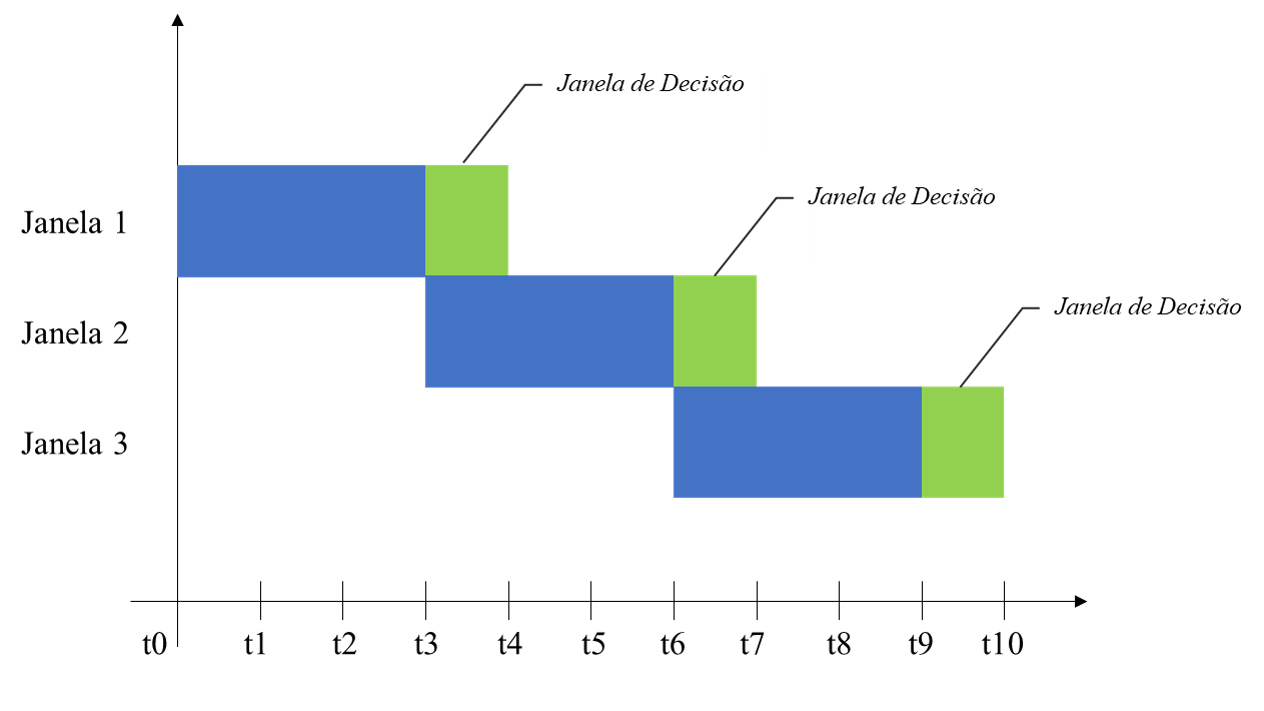
\includegraphics[width=15cm]{dados-agrupados.png}
                \centering
            \end{figure}
      
        \section{Estratégia de Compra e Venda}\label{sec:estrategia-saida}
            \paragraph{}De modo a facilitar a tomada de decisão e diminuir as premissas tomadas pelo agente autônomo, optou-se por uma estratégia que desconsidera a quantidade de ações possuídas. A função do robô reduz-se, portanto, a detectar movimentações de alta dos preços para que se possa obter lucro comprando e vendendo, necessariamente nessa ordem, sem guardar excedentes de ações ou papéis de uma janela de tempo para outra. 
            
            \paragraph{}Uma das possíveis estratégias para a geração de um indicador direcional de alta dos preços é assumir que se a diferença entre o máximo preço negociado na janela de previsão e o preço de fechamento da janela de tempo superar um limite $x$, o agente autônomo deve enviar uma ordem de compra no período $t$ e uma ordem de venda no período $t+t'$, assim como proposto em \citet{everton-silva-master}. O principal problema dessa abordagem é que, para um resultado positivo a longo prazo, o modelo precisa garantir uma precisão apurada para que os ganhos superem as possíveis perdas, classificadas como falsos positivos pelo modelo. Esses falsos positivos, ou seja, baixas de preço erroneamente classificadas como altas, podem gerar um prejuízo desproporcional se ordens de compra e venda forem enviadas a mercado no ínicio e no fim de cada janela de previsão para um cenário de queda abrupta dos preços.
            
            \paragraph{}Com o objetivo de contornar os possíveis cenários de perda descritos acima, foi necessária a elaboração de uma estratégia que considerasse outros fatores na variação de preço dentro da janela de previsão. Dessa maneira, para gerar o indicador de compra, é verificado se a primeira variação positiva de $x$ entre preço negociado e preço de fechamento ocorreu antes da primeira variação negativa $y$. Se ocorrer essa situação, será feita a sinalização de compra para o modelo. No cenário de um falso positivo, nessa abordagem, estabelece-se que uma ordem de venda a mercado será enviada se a diferença entre o preço de fechamento e a última negociação superar o valor $y$. Se, por acaso, o preço não ultrapassar o limite entre $x$ e $-y$, a ordem de venda a mercado será enviada ao final da janela de previsão.
            
            \begin{figure}[h]
                \caption{Exemplo de situação de não-compra}
                \label{img:estrategia-saida}
                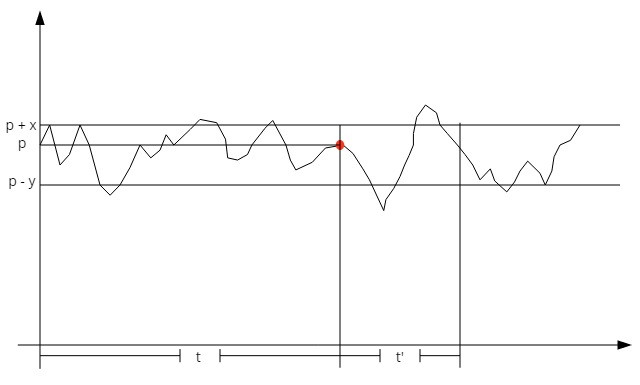
\includegraphics[width=13cm]{estrategia-saida1.png}
                \centering
            \end{figure}
            
            \paragraph{}Para ilustrar uma situação de não-compra, observa-se a imagem \ref{img:estrategia-saida}, que representa a variação dos preços ao longo do tempo. Mesmo o preço tendo ultrapassado o limite superior $p + x$ ao fim do intervalo $t'$, a saída indicando o sinal de compra não é gerada porque o limite inferior $p - y$ foi ultrapassado anteriormente.
            
            \paragraph{}Destaca-se, nessa abordagem, que o maior prejuízo que pode ser obtido por um falso positivo é de y. É válido mencionar também que nem todo falso positivo, nessa perspectiva, causará prejuízo. Na situação em que o preço de fechamento supera o valor de abertura em $z$, sendo $z < x$, é possível obter lucro sem que o sinal direcionador de compra seja disparado.
            
        \section{Geração do sinal de saída}
            \paragraph{}Dada a estratégia definida na seção anterior, conclui-se que trata-se de um problema de classificação: se o preço tiver variação positiva maior do que $x$, tem-se a saída do modelo com o valor 1, o que significa que ordens de compra e venda serão enviadas conforme definido na seção anterior. Se a variação de preço for positiva mas não ultrapassar o limite superior $x$ ou se a variação for negativa, tem-se a saída com o valor $1$.
            
            \paragraph{}Dessa forma, o problema reduz-se a um classificador binário, em que temos somente 2 classes possíveis para serem previstas.
            
    \chapter{Modelos de Previsão e Técnicas de Validação}
    
        \paragraph{}Nesse capítulo são definidos os modelos utilizados para o treinamento e previsão, assim como as técnicas de validação utilizadas para o levantamento de precisão e das oportunidades de compra corretamente aproveitadas pelo preditor.
        
        \section{Modelos Utilizados}\label{sec:models}
        
            \paragraph{}São definidos abaixo os modelos utilizados para treinamento e previsão do conjunto de dados.
        
            \subsection{MLP (\textit{Multi-layer Perceptron})}
            
                \paragraph{}Segundo a definição de \citet{scikit-learn}, essa técnica trata-se de um algoritmo de aprendizado profundo supervisionado que é capaz de aprender uma função $f(\cdot) : R^m \xrightarrow{}R^o$ pelo treinamento sobre um conjunto de dados, sendo $m$ o número de dimensões de entrada (variáveis do conjunto de treino) e $o$ o número de dimensões da saída. Dadas uma combinação de variáveis de entrada $X = x_1, x_2, ..., x_m$ e um alvo de saída $y$, o modelo é capaz de aprender uma função de aproximação não-linear tanto para regressão quanto para classificação, sendo esse último o problema a ser resolvido nesse projeto. Entre a camada de entrada e a camada de saída podem existir uma ou mais camadas não lineares, chamadas de camadas escondidas. Ilustra-se o MLP a partir da figura \ref{img:mlp-example}:
                
                \begin{figure}[h]
                    \caption{MLP com uma camada escondida entre a camada de entrada e a de saída}
                    \label{img:mlp-example}
                    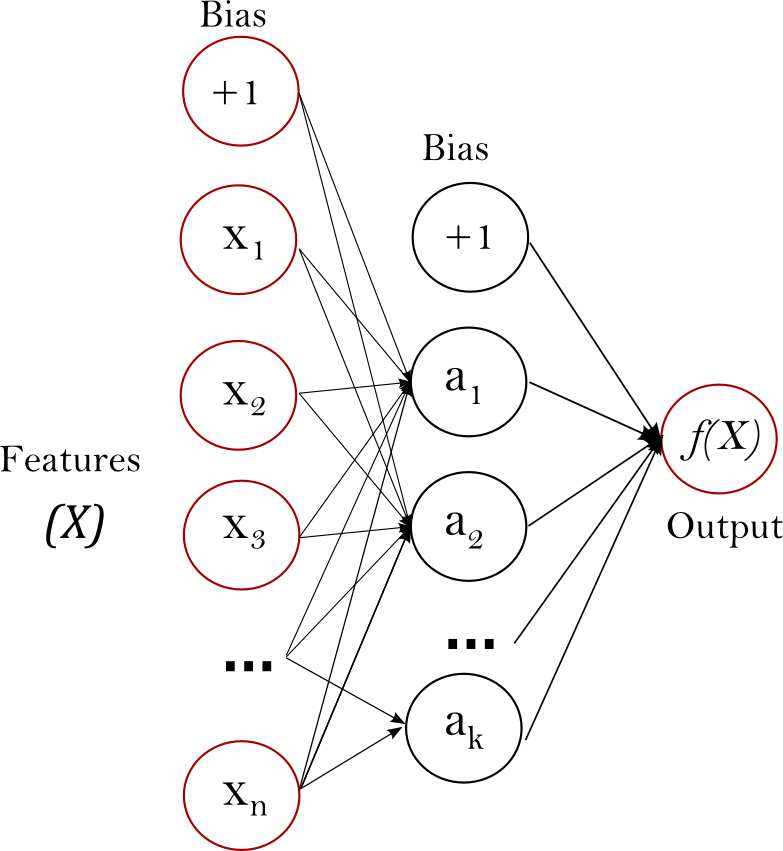
\includegraphics[width=7cm]{mlp-example.png}
                    \centering
                \end{figure}
                
                \paragraph{}Cada círculo na camada de entrada contém o que é chamado de neurônio $\{x_i|x_1,x_2,...,x_m\}$ e cada círculo da camada escondida representa um neurônio da camada escondida e transforma os valores da camada anterior baseado em uma soma com pesos $w_1x_1 + w_2x_2 + ... + w_mx_m$, seguido por uma função de ativação não linear $g(\cdot) : R \xrightarrow{} R$. A camada de saída recebe os valores da última camada escondida e transforma nos valores de saída \cite{mlp-model}.
                
            \subsection{Regressão Logística}
            
                \paragraph{}A regressão logística pode ser definida como uma técnica para calcular os parâmetros de um modelo logístico, ou seja, um modelo que se utiliza de funções logísticas para modelar o valor de uma variável binária dependente. Dessa maneira, essa técnica é vastamente utilizada para problemas de classificação cujas classes a serem previstas podem assumir 2 valores possíveis, como uma decisão de compra e não-compra de ações no mercado financeiro, escopo delimitado pelo projeto. A imagem \ref{img:logreg-example} ilustra os passos para a previsão da saída pelo algorítmo.
                
                \begin{figure}[h]
                    \caption{Regressão logística}
                    \label{img:logreg-example}
                    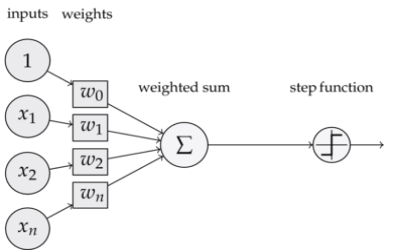
\includegraphics[width=10cm]{logreg-example.png}
                    \centering
                \end{figure}
                
                \paragraph{}Assim como no MLP (\ref{img:mlp-example}), a Regressão Logística aplica pesos às variáveis de entrada para encontrar uma soma calculada das mesmas. Em seguida, ao invés de passar por camadas escondidas, essa soma passa por uma função de atachamento que retorna uma probabilidade associada. Essa probabilidade, por fim, passa por uma função degrau que classifica a saída baseado em um limiar \cite{logreg-model}.
                
                \paragraph{}No modelo logístico, o logarítmo de acerto (referente à saídas classificadas como "1") é uma combinação linear de uma ou mais variáveis independentes binárias ou contínuas, que são as entradas do modelo. A probabilidade correspondente ao valor "1", pode variar continuamente entre 0 e 1 e a função que traduz essa probabilidade para a a classe final é chamada de função logística.
                
        \section{Técnicas de Validação}\label{sec:validation}
        
            \paragraph{}Nessa seção são descritas as técnicas de validação usadas para o projeto.
            
            \subsection{Janelas Deslizantes}
            
                \paragraph{}Como o problema é de séries de tempo, a divisão do conjunto de dados entre treinamento e teste foi feita de modo que, obrigatoriamente, o conjunto de testes fosse composto por dados obtidos cronologicamente depois dos dados de treino. Dessa forma, foi possível obter previsões mais próximas do cenário real, em que a entrada do modelo obedece uma ordenação temporal.
                
                \paragraph{}Com o objetivo de obter o maior aproveitamento possível de dias utilizados para treino e previsão do conjunto de dados, foi utilizada a técnica de janelas deslizantes de treino e previsão. Nessa estratégia, utiliza-se um número $N$ de dias para formar o conjunto de treino e um número $N'$ para o conjunto de testes para realizar a validação. Na próxima iteração, utiliza-se o mesmo número de dias para as duas janelas, com a diferença que a janela de treino e de previsão tem início e fim do início e fim anteriores. A imagem \ref{img:sliding-validation} pode ser usada para ilustrar a explicação.
                
                
                \begin{figure}[h]
                    \caption{Janelas deslizantes com 4 dias usados para o conjunto de treino e 1 dia para o conjunto de teste}
                    \label{img:sliding-validation}
                    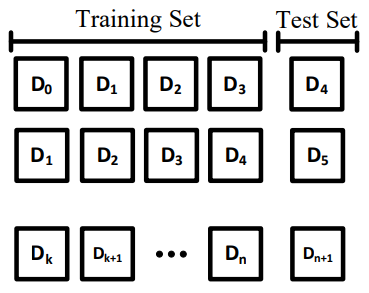
\includegraphics[width=8.3cm]{sliding-validation.PNG}
                    \centering
                \end{figure}
                
            \subsection{Expansão das Janelas Deslizantes}
            
                \paragraph{}Com o intuito de encontrar o número ótimo de dados de treino necessários para o modelo, foi feita uma iteração tal que, ao final do ciclo de janelas deslizantes de $N$ dias de treino, fosse iniciado um outro ciclo com $N+1$ dias para o conjunto de treino. Foi utilizada a linguagem de programação \textit{Python} para a implementação dessa lógica.
                
            \subsection{Parâmetros de validação}
            
                \paragraph{}Para cada previsão feita pelo modelo, cria-se uma matriz de confusão (\ref{img:matriz-confusao}) antes de extrair os parâmetros utilizados para mensurar a perfomance do modelo. 
                
                \begin{figure}[h]
                    \caption{Matriz de confusão}
                    \label{img:matriz-confusao}
                    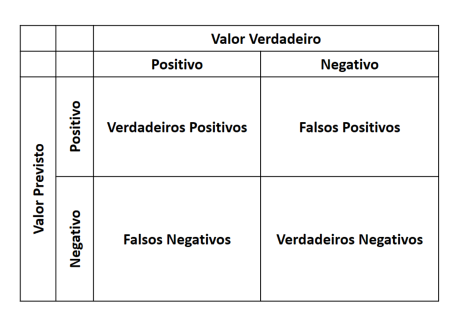
\includegraphics[width=10cm]{matrix-confusao.png}
                    \centering
                \end{figure}
                
                \paragraph{}Com a matriz de confusão, pode-se visualizar de forma mais direta os valores previstos em relação aos valores verdadeiros. Dessa forma, são de interesse para a performance do modelo o número de verdadeiros positivos e verdadeiros negativos em relação ao resto do conjunto.
                
                \paragraph{}Um verdadeiro positivo é quando uma classe classificada como "1" no conjunto de testes de fato possui o valor verdadeiro "1". Um falso positivo, por sua vez, refere-se a uma classe que é classificada como "1" enquanto possui "0" como valor verdadeiro. Pensamento análogo pode ser aplicado aos verdadeiros negativos e falsos negativos.
                
                \paragraph{}Para o domínio do trabalho, tem-se como interesse óbvio um modelo que seja capaz de obter mais acertos do que erros para obter lucro e, além disso, identifique o maior número possível de oportunidades de compra. A a matriz de confusão pode ser reaproveitada para gerar os parâmetros de validação abaixo.
                
                \subsubsection{Revocação}
                    \paragraph{}A revocação é definida como a quantidade de valores classificados corretamente como verdadeiros sobre a quantidade total de verdadeiros do conjunto de teste. Pode ser calculada pela fórmula abaixo:
                    
                    \begin{equation}
                        R = \frac{VP}{VP + FN} = \frac{VP}{TP}
                    \end{equation}
                    
                    \paragraph{}Onde R é a revocação, FN é a quantidade de amostras classificadas como falso negativas e TP é o total de valores positivos do conjunto de teste.
                    
                \subsubsection{Precisão}
                    \paragraph{}A precisão é definida como a quantidade de valores classificados corretamente como verdadeiros sobre a quantidade total de previsões verdadeiras do conjunto de teste. Pode ser calculada pela fórmula abaixo:
                    
                    \begin{equation}
                        P = \frac{VP}{VP + FP}
                    \end{equation}
                    
                    \paragraph{}Onde P é a precisão e VP e FP são classificadas como as amostras classificadas como verdadeiros positivos e falsos positivos, respectivamente.
                    
                \paragraph{}Para cada ciclo de uma determinada janela de treinamento, é calculada a média das precisões e das realocações obtidas de forma a obter a melhor combinação de dias de treino. Quanto mais alta a média das precisões, mais alta é a taxa de acerto obtida para futuras amostras. Se a realocação estiver alta, significa que o modelo está identificando grande parte das oportunidades de compra. Nesse ponto, é possível escolher a estratégia a ser seguida: manter um modelo mais seguro, que tenha menos sensibilidade para a hora de entrar no mercado, porém com maiores chances de acerto; manter um modelo mais agressivo, que seja mais sensível para identificar oportunidades, porém menos preciso em sua previsão.
                
                \paragraph{}Estendendo a análise da precisão aplicada na estratégia definida na seção \ref{sec:estrategia-saida}, é possível identificar imediatamente um mínimo de precisão segura, baseado nos limites superior $x$ e inferior $y$, que o modelo deve alcançar para o cenário de prejuízos máximos. Um cenário de prejuízo máximo, como discutido no capítulo anterior, se caracteriza quando todas as previsões classificadas como falso positivas alcançam o limite inferior $y$, causando um prejuízo de $N \cdot Y$, sendo $N$ o número de papéis negociados. 
                
                \paragraph{}Supondo que, para obter lucro, o volume de verdadeiros positivos vezes o lucro precisa ser maior do que o volume de falsos positivos vezes a perda, tem-se a seguinte relação:
                
                \begin{equation}
                    V \cdot P \cdot x \geq V \cdot (1 - P) \cdot y
                \end{equation}
                
                \paragraph{}Onde $V$ é o volume de papéis negociados, $P$ é a precisão de acerto e $x$ e $y$ referem-se aos limites superiores e inferior, respectivamente. Estabelecendo que a relação de $x$ e $y$ ocorre por $K = \frac{x}{y}$, a equação pode ser reduzida a:
                
                \begin{equation}
                    K > \frac{1}{P} - 1
                \end{equation}
                
                \paragraph{}E:
                
                \begin{equation}
                    K + 1 > \frac{1}{P}                    
                \end{equation}
                
                \paragraph{}Então:
                
                \begin{equation}\label{eq:precisao-minima}
                    P > \frac{1}{K + 1}
                \end{equation}
                
                \paragraph{}Em suma, a partir da relação acima, pode ser definida uma precisão mínima que nunca causa prejuízos nos falsos positivos a partir dos limites $x$ e $y$. Destaca-se o cenário de que, mesmo obtendo uma precisão menor do que a mínima segura, ainda é possível obter lucro pelo modelo se houver uma parcela de falsos positivos que não ultrapassagem a margem inferior $y$.
                
                
                
    \chapter{Resultados e Discussões}
    
        \paragraph{}Como estudo de caso para o projeto, foi escolhida a análise sobre a PETR4, ações preferências da Petrobrás, empresa que voltou a ocupar em outubro de 2018 o título de mais valiosa do Brasil, chegando a bater a marca de R\$358 bilhões \cite{petr4-intro}. 
        
        \paragraph{}Para isso, foram importados todos os dados diários negociados da BM\&FBOVESPA de julho de 2018 até janeiro de 2019 e feito o pré-processamento descrito na seção \ref{sec:grouping}.
        
        \paragraph{}Após a importação dos dados brutos, escolheu-se empricamente uma janela de tempo de 3 minutos para a geração os indicadores de análise técnica com a saída determinada pela estratégia descrita na seção \ref{sec:estrategia-saida} para o intervalo futuro de tempo de 1 minuto a partir do tempo de fim da janela de tempo. 
        
        \paragraph{}Para o limite superior e inferior dos preços, também utilizados na estratégia de formação da variável de saída, foram considerados o valores $x = 0,01$ e $y = 2x = 0,02$, respectivamente. A escolha desses limites está intrinsecamente ligada com a distribuição das classes binárias "0" e "1" do conjunto de dados e, para esses limites, foi possível obter uma distribuição de $55,63\%$ da classe "1". A distribuição das classes próxima de $50\%$ é essencial, pois reduz o viés que pode ser obtido decorrente de uma distribuição desproporcional dos dados. O detalhamento de outros parâmetros como períodos de tempo para formação de cada indicador está especificado no apêndice \ref{cap:params}. Especificados os parâmetros de pré-processamento, o software C\# inicia o agrupamento dos dados para cada dia coletado na BM\&FBOVESPA.
        
        \paragraph{}Após o pré-processamento dos dados e normalização das variáveis, observou-se a correlação entre as variáveis de entrada e a variável de saída pelo mapa de calor representado pela figura \ref{img:heatmap}. Observa-se que, apesar das variáveis independentes de entrada possuirem uma correlação forte entre si em vários casos, a correlação dessas variáveis com a variável dependente de saída é fraca, alcançando seu maior valor com a variável que representa o número de negociações dentro do intervalo especificado. 
        
        \begin{figure}[h]
            \caption{Mapa de Calor das Correlações entre as Variáveis}
            \label{img:heatmap}
            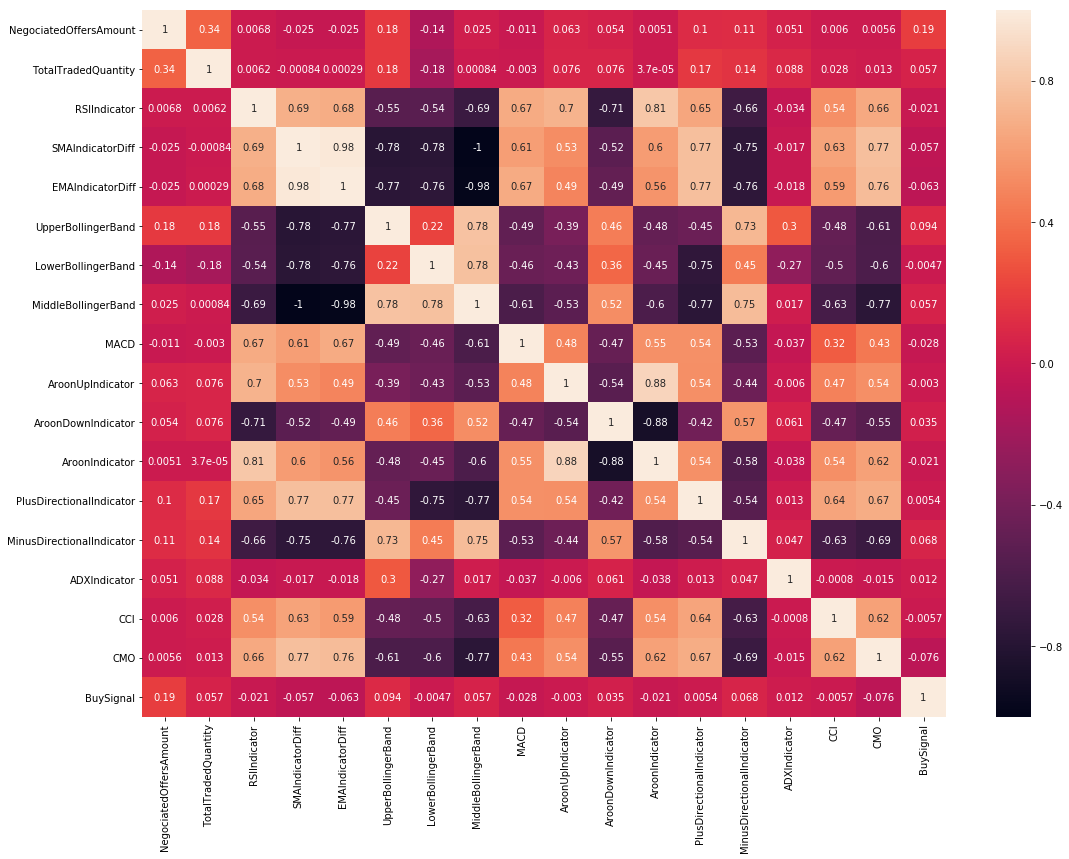
\includegraphics[width=15cm]{corr.png}
            \centering
        \end{figure}
        
        São aplicados, então, os modelos de Regressão Logística e \textit{Multi-layer Percerptron} descritos em \ref{sec:models} para janela de treino, como detalhadado em \ref{sec:validation}. As figuras \ref{img:performance-logreg} e \ref{img:performance-mlp} mostram a performance de cada modelo com a medida das precisões e realocações sobre a quantidade de dias de treino. Dessa forma, é possível acompanhar a evolução das medidas até o máximo de cada métrica.
        
        \paragraph{}Em ambos os gráficos, nota-se que tanto as realocações quanto as precisões apresentam uma curva ascendente até alcançarem o seu máximo, depois apresentam uma curva descendente. Na Regressão Logística, a máxima realocação observada foi de aproximadamente $90,56\%$ com 88 dias de treino e a máxima precisão foi de aproximadamente $63,07\%$, alcançada com 78 dias. Já no MLP, foi observada uma realocação máxima de aproximadamente $90,22\%$ com 80 dias, enquanto que sua maior precisão foi de $63,28\%$ com 98 dias de treino.
        
        \begin{figure}[h!]
            \caption{Performance da Regressão Logística}
            \label{img:performance-logreg}
            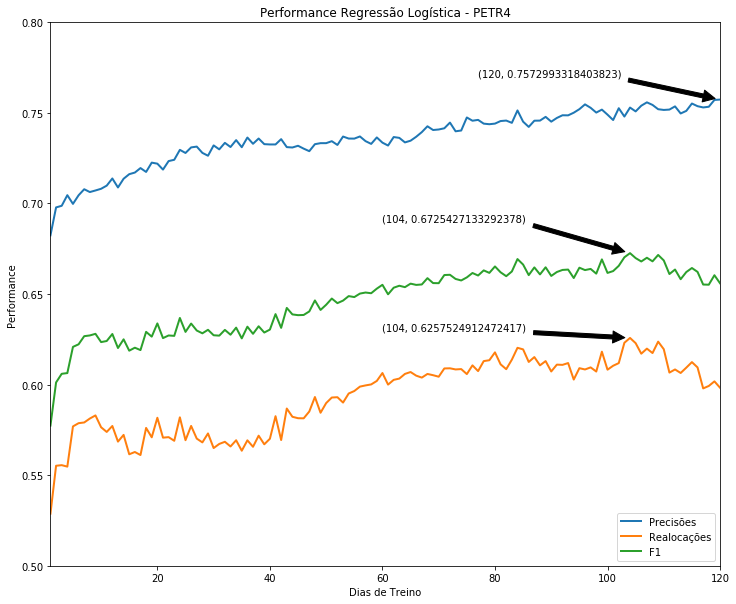
\includegraphics[width=12cm]{performance-logreg.png}
            \centering
        \end{figure}
        
        \begin{figure}[h!]
            \caption{Performance do \textit{Multi-layer Perceptron}}
            \label{img:performance-mlp}
            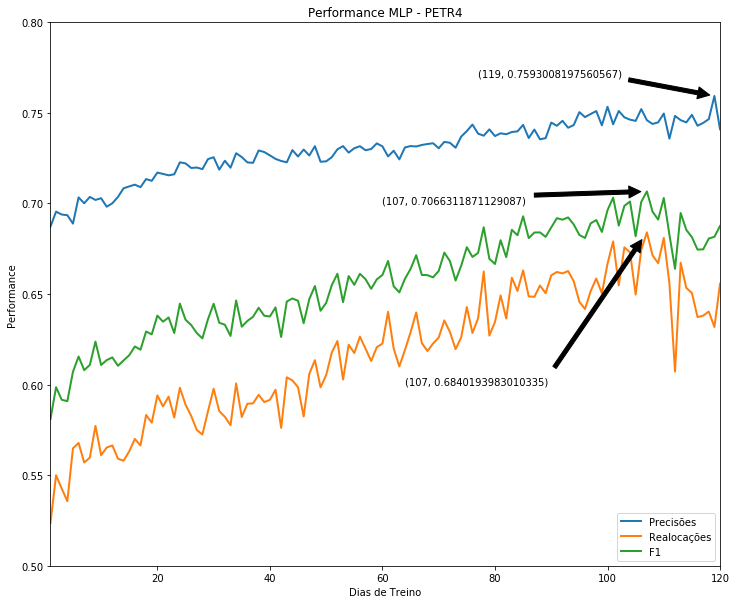
\includegraphics[width=12cm]{mlp-performance.png}
            \centering
        \end{figure}
        
        \paragraph{}Apesar da maior precisão encontrada pelos modelos ter sido obtida com o \textit{Multi-Layer Perceptron}, o modelo necessitou de um conjunto de dados dos últimos 98 dias, 20 dias a mais do que o algoritmo de Regressão Logística necessitou para encontrar seu máximo de precisão. Para a realocação, o MLP necessitou de 8 dias a menos de treino para alcançar seu máximo de $90,22\%$, porém o maior valor, de $90,46\%$, foi alcançado pela Regressão Logística com 88 dias de treino.
        
        \paragraph{}Ao observar a evolução das precisões e realocações, pode-se perceber um ruído muito maior no MLP. A curva traçada para ambas as medidas pela regressão é consideravelmente mais suave, fator que indica maior estabilidade e, portanto, confiabilidade e poder preditivo do algoritmo.
        
        \paragraph{}Nota-se que a maior precisão obtida pelos modelos utilizados, de $63,28\%$, ainda encontra-se abaixo da mínima precisão segura definida na equação \ref{eq:precisao-minima}. Para garantir a máxima segurança do modelo, segundo essa relação, seria preciso alcançar pelo menos $66,67\%$ de precisão. Apesar disso, dada a proximidade da precisão real com a mínima segura, é plausível a elaboração de uma estratégia mais arrojada que considere puramente o sinal de saída do presente modelo como disparador de ordens de compra e venda devido a improbabilidade de existir uma parcela elevada de falsos positivos com máximo prejuízo.
        
  
  \chapter{Conclusões}
  
    \section{Conclusões Gerais}
    
        \paragraph{}O presente trabalho teve como objetivo aplicar técnicas de aprendizado de máquina para gerar modelos de previsão de direção dos preços. A partir da validação utilizando testes históricos das séries temporais, foi possível verificar que a tomada de decisão apoiada por algoritmos de inteligência artificial pode ser muito mais eficaz do que uma simples análise técnica tradicional.
        
        \paragraph{}Ao aplicar a estratégia definida para o caso de uso real das ações da Petrobrás (PETR4), foi possível observar que, mesmo para um grupo mínimo de dias de treino, o modelo apresentou uma precisão considerávelmente maior do que um modelo aleatório. Apesar do caso de uso não apresentar o requisito mínimo de precisão para garantir o lucro, já é possível a utilização do presente modelo para uma estratégia mais arrojada puramente baseada em aprendizado de máquina.
        
        \paragraph{}Mesmo restringindo o caso de uso à análise de um ativo específico da BM\&FBOVESPA, o agrupamento dos dados foi implementado com o objetivo de ser generalizado para todo o conjunto de dados de negociação em uma base diária de \textit{ticks}, incluindo mini-índices e opções. A flexibilização pensada no \textit{software} implementado para a geração dos indicadores de análise técnica também oferece a possibilidade de customização e adaptação para ativos de outra natureza de flutuação, permitindo análises adequadas aos mais diversos fatores que regem a oscilação dos preços de uma ação.
        
    \section{Trabalhos Futuros}
        
        \paragraph{}Em relação ao conjunto de dados de entrada do modelo de predição, nota-se uma predominância muito maior de indicadores técnicos aplicados puramente ao dados provenientes do conjunto de dados negociados. Com o objetivo de aprofundar a análise para considerar a volatilidade de um ativo, torna-se interessante a consideração das informações do livro de ofertas para a criação de variáveis com informações sobre a quantidade de ordens de compra e venda em um intervalo, o valor dessas ordens e outras características.
        
        \paragraph{}Em relação ao agrupamento dos dados, foi utilizada uma abordagem por separação de janelas de tempo e previsão de forma que uma janela de tempo nunca colidisse com a outra. Por causa disso, a implementação de janelas deslizantes no tempo podem ser úteis para aumentar a quantidade de dados adquiridos para o treinamento do modelo.
        
        \paragraph{}Para consumo diário de um agente autônomo responsável pelas negociações, ainda é necessária a aquisição manual dos dados nos servidores públicos da BM\&FBOVESPA e posterior execução do \textit{software} desenvolvido para o pré-processamento. Neste caso, uma solução de agendamento que recorrentemente verificasse a disponibilização de novos arquivos de negociação seguida de um pré-processamento e agrupamento dos mesmos poderia automatizar esse esforço.
        
        \paragraph{}Após treinado o modelo com os dados agrupados, torna-se necessária a exposição de um serviço que retorne o sinal de previsão do próximo intervalo baseado nas entradas de indicadores de análise técnica descritos ao longo do trabalho. Para garantir a disponibilidade desse serviço, torna-se interessante a hospedagem do mesmo em algum provedor de nuvem como \textit{Amazon Web Services} ou \textit{Google Cloud Computing}. A lógica a ser executada a cada requisição, dessa maneira, seria a predição desses dados de entrada em um modelo já treinado, salvo em um arquivo binário e carregado em memória para executar imediatamente as previsões.
  

  \backmatter
  \bibliographystyle{coppe-unsrt}
  \bibliography{example}

  \appendix 
  \chapter{Parâmetros de calibração}\label{cap:params}
  
    \paragraph{}Na lista abaixo, estão presentes todos os parâmetros de podem ser calibrados na geração de dados agrupados. Além dos períodos para os indicadores de análise técnica, também é possível selecionar o tamanho das janelas de tempo e previsão e limites superiores e inferiores para estruturar a estratégia de compra e venda.
  
    \begin{listing}
    \begin{minted}[frame=single,
                   framesep=3mm,
                   linenos=true,
                   xleftmargin=21pt,
                   tabsize=4]{js}
    {
      "negFolderPath": "C:\\MarketData\\Bovespa\\",
      "buyFolderPath": "C:\\MarketData\\AllData\\",
      "sellFolderPath": "C:\\MarketData\\AllData\\",
      "negFilePrefix": "NEG_",
      "buyFilePrefix": "OFER_CPA_",
      "sellFilePrefix": "OFER_VDA_",
      "dateSuffixFormat": "yyyyMMdd",
      "instrumentSymbol": "PETR4",
      "slidingWindowMinutes": 3,
      "RSIPeriods": 14,
      "SMAPeriods": 14,
      "BollingerBandsPeriods": 14,
      "BuyTimeHold": 1,
      "CsvCharSeparator": ",",
      "PeriodsToNormalize": 28,
      "OutputCsvPath": "C:\\Projects\\GitHub\\stock-analysis\\",
      "ShortMACDPeriods": 12,
      "LongMACDPeriods": 26,
      "AroonIndicatorPeriods": 14,
      "ConsiderOrderFiles": false,
      "InterpolateWindows": false,
      "IndexStockCodeVariation": false,
      "ATRPeriods": 14,
      "CMOPeriods": 14,
      "ROCPeriods": 1,
      "MinimumVariationOfInterest": 0.01
    }
    \end{minted}
    \caption{Arquivo JSON com propriedades de calibração dos indicadores de análise técnica} 
    \label{json-example}
    \end{listing}
\end{document}
%% 
%%
%% End of file `example.tex'.
